\section{AXI Protocol}

\subsection{Introduction}
The AXI protocol is organized into five independent channels, each with its own handshake mechanism for reliable communication:

\begin{multicols}{2}
\begin{figure}[H]
    \centering
    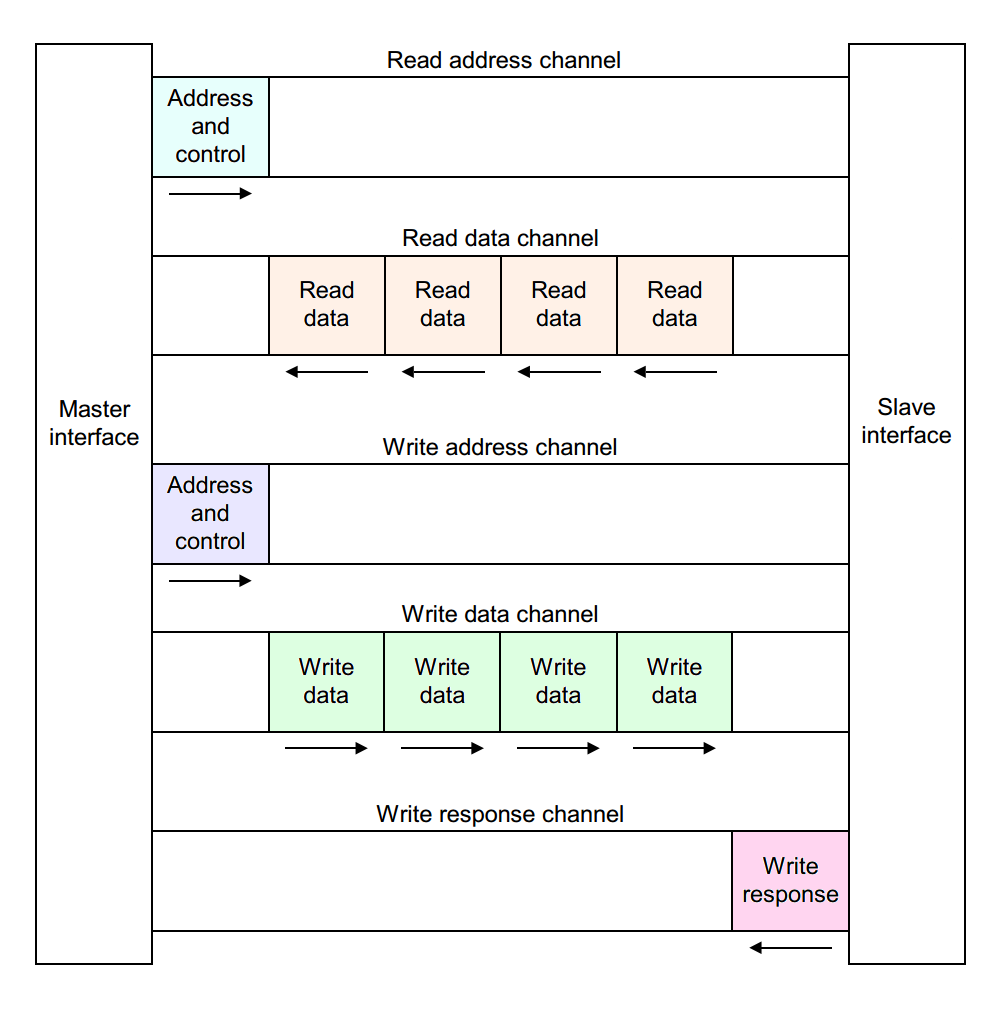
\includegraphics[width=1\linewidth]{images/axi/axi_channels.png}
    \caption{AXI Channels}
\end{figure}

\begin{itemize}
    \item Read Address Channel (\textbf{AR}): Used by the master to send read address and control information to the slave.

    \item Read Data Channel (\textbf{R}): Used by the slave to return read data and response information to the master.

    \item Write Address Channel (\textbf{AW}): Used by the master to send write address and control information to the slave.

    \item Write Data Channel (\textbf{W}): Used by the master to send write data to the slave.

    \item  Write Response Channel (\textbf{B}): Used by the slave to send a write response to the master. 
\end{itemize}

These channels operate independently, allowing for concurrent read and write operations. 
\end{multicols}



\subsubsection{Transaction \& Transfer}
A transaction in AXI refers to a complete operation initiated by a master, which can involve multiple transfers.

A transaction typically consists of:

\begin{itemize}
    \item A request phase: The master sends the address and control information to the slave.

    \item  A data phase: The master and slave exchange data (one or more transfers).

    \item A response phase: The slave sends a response to the master indicating the status of the transaction (success, error...).
\end{itemize}

There is two types of transactions:
\begin{itemize}
    \item Read Transaction: The master reads data from the slave.
    \item Write Transaction: The master writes data to the slave.
\end{itemize}

\subsection{Handshake}

In the AXI protocol, communication between the master and slave is based on a handshake mechanism. Each channel has its own handshake signals, which allow the master and slave to coordinate the transfer of information.

\subsubsection{Handshake Signals}
Every AXI channel uses two signals for handshaking:

\begin{itemize}
    \item \code{VALID}: Indicates that the sender (master or slave) has valid data or control information to transfer. 
    \item \code{READY}: Indicates that the receiver (slave or master) is ready to accept the data or control information. 
\end{itemize}
        
The transfer of information occurs only when both \code{VALID} and \code{READY} are high at the same time.

\subsubsection{Handshake Rules}
\begin{itemize}
    \item  \code{VALID} must not depend on the \code{READY} signal.
    \item  \code{READY} can depend on the \code{VALID} signal.
    \item   Once \code{VALID} is asserted, it must remain high until the transfer completes.
    \item  \code{READY} can be asserted before or after \code{VALID} is asserted.
\end{itemize}

    

   

    

\begin{figure}[H]
    \centering
    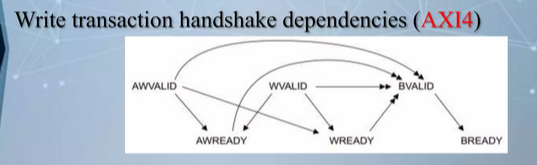
\includegraphics[width=\linewidth]{images/dependency.png}
    \caption{Handshake Dependency AXI 4}
\end{figure}

\begin{figure}[H]
    \centering
    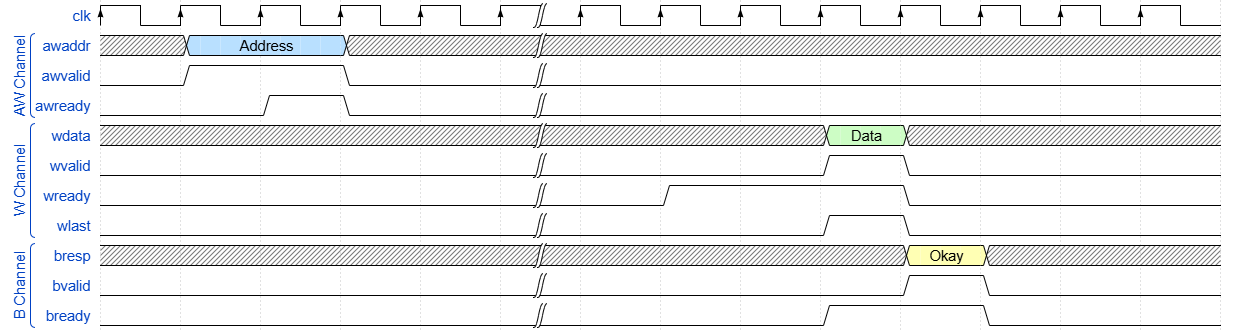
\includegraphics[width=\linewidth]{images/axi/axi_single_write.png}
    \caption{AXI Write single transaction}
\end{figure}

\begin{figure}[H]
    \centering
    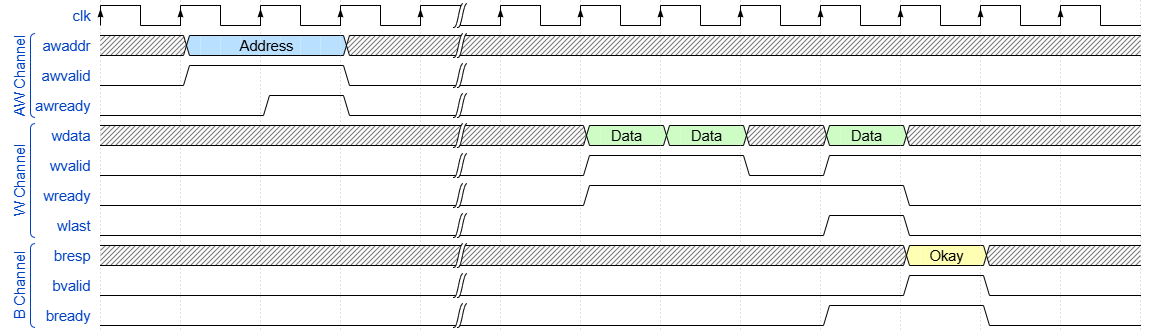
\includegraphics[width=\linewidth]{images/axi/axi_single_write_multiple.png}
    \caption{AXI Write multiple transaction}
\end{figure}

\newpage
\subsection{Addresses} \label{Addresses}

The address calculation during a transaction depends on the Burst Mode used.

\begin{table}[H]
\begin{threeparttable}
\caption{Burst Modes}
\begin{tabularx}{\linewidth}{X | X | X | X | X}
Burst Mode                  & FIXED & INCR & BURST & RESERVED \\ 
\hline        
\mintinline{vhdl}{aXaddr}   & "00"  & "01" & "10"  & "11"     \\
\end{tabularx}
\end{threeparttable}
\end{table}

\textbf{Note}: If the \mintinline{vhdl}{burst_length} is set to 0, there is no differences between FIXED, INCR and WRAP mode.

\subsubsection{Burst Mode Fixed}

In fixed mode, the \mintinline{vhdl}{awaddr} address remains the same for every transfer in the burst.

\subsubsection{Burst Mode INCR}

In mode INCR, the \mintinline{vhdl}{aXaddr} for each transfer in the burst is incremented by the size of the transfer.

$$Address_n = Address_0 + (n \cdot BurstSize)$$

where:
\begin{itemize}
    \item $Address_n$ is the address for the $n$-th transfer.
    \item $n$ is the transfer index (starting from 0).
    \item $BurstSize$ is the number of bytes per transfer.
\end{itemize}

\textbf{Note:} The start address of a burst must align with the burst size to ensure that the address increments correctly for each transfer.

For example: If the burst size is 4 bytes, the start address must be aligned to a 4-byte boundary (the lower 2 bits of the address must be 0).

\subtitle{Burst Size}

The burst size can be 1 byte, 2 bytes, 4 bytes, 8 bytes, 16 bytes, 32 bytes, 64 bytes, or 128 bytes.

\subtitle{Burst Length}
For INCR bursts, the burst length can range from 1 to 256 transfers.

\subtitle{Example}

\begin{multicols}{2}
\begin{itemize}
    \item $StartAddress = 0x1000$
    \item $BurstSize = 2 \Leftrightarrow \SI{4}{\byte}$ \TODO{Explain Burst Size}
    \item $BurstLength = 3 \Leftrightarrow 4$ transfers
\end{itemize}

\begin{table}[H]
\begin{threeparttable}
\caption{INCR mode Address calculation}
\begin{tabularx}{\linewidth}{wm{0.5\linewidth} | wm{0.5\linewidth}}
\hline
\textbf{Transfer}   & \textbf{Address} \\ 
\hline        
Transfer 0 & 0x1000 \\
Transfer 1 & 0x1004 \\
Transfer 2 & 0x1008 \\
Transfer 3 & 0x100C \\
\hline
\end{tabularx}
\end{threeparttable}
\end{table}
\end{multicols}

\newpage
\subsubsection{Burst Mode WRAP}

In mode WRAP, the \mintinline{vhdl}{aXaddr} increments like in INCR mode but it wraps around to a lower address after reaching a boundary defined by the burst size and burst length.

\subtitle{Burst Size}
The burst size can be 1 byte, 2 bytes, 4 bytes, 8 bytes, 16 bytes, 32 bytes, 64 bytes, or 128 bytes.

\subtitle{Burst Length}
For WRAP bursts, the burst length must be 2, 4, 8, or 16 transfers. The burst length must be a power of 2.

\subtitle{Address Calculation}
The address for each transfer in a WRAP burst is calculated as follows:

$$WrapBoundary = StartAddress + (BurstLength \cdot BurstSize)$$

where:
\begin{itemize}
    \item $StartAddress$: The initial address of the burst.
\end{itemize}

The address increments by the burst size for each transfer.

When the address reaches the wrap boundary, it wraps around to the start of the boundary.

\subtitle{Example}
\begin{itemize}
    \item $StartAddress = 0x1004$
    \item $BurstSize = 2 \Leftrightarrow \SI{4}{\byte}$ 
    \item $BurstLength = 3 \Leftrightarrow 4$ transfers
    \item $WrapBoundary = 0x1004 + (4 \cdot 4) = 0x1014$
\end{itemize}

\begin{table}[H]
\begin{threeparttable}
\caption{WRAP mode Address calculation}
\begin{tabularx}{\linewidth}{wm{0.5\linewidth} | wm{0.5\linewidth}}
\hline
\textbf{Transfer}   & \textbf{Address} \\ 
\hline        
Transfer 0 & 0x1004 \\
Transfer 1 & 0x1008 \\
Transfer 2 & 0x100C \\
Transfer 3 & 0x1010 \\
Transfer 4 & 0x1004 \\
\hline
\end{tabularx}
\end{threeparttable}
\end{table}

Transfer 4 Address would be 0x1014, but it wraps around to 0x1004.

\subsubsection{Burst Mode RESERVED}
The RESERVED burst type in AXI is a placeholder for future extensions or custom implementations.

If encountered, it should be treated as an error or handled according to custom implementation rules.

\subsubsection{Burst Size}
The burst size determines the number of bytes transferred in each beat of the burst. It is specified by the \mintinline{vhdl}{ARSIZE} or \mintinline{vhdl}{AWSIZE} signal (for read and write transactions, respectively). 

The burst size width is 3 bits and it is calculated with this formula:

$$BurstSize = 2^{BurstSizeValue} \si{\byte}$$


\subsubsection{Burst Length}
